\documentclass{article}

\usepackage{graphicx}
\usepackage{wrapfig}
\usepackage{subcaption}
\usepackage[margin=1in]{geometry}
\usepackage{amsmath} % or simply amstext
\usepackage{amssymb}
\usepackage{siunitx}
\usepackage{booktabs}
\usepackage[export]{adjustbox}
\newcommand{\angstrom}{\textup{\AA}}
\newcommand{\colormap}{jet}  % colorbar to use
\usepackage{cleveref}
\usepackage{booktabs}
\usepackage{gensymb}
\usepackage{float}
\usepackage{xr}

\externaldocument[M-]{Draft}

\title{Supporting Information: Statistical Inference of Transport Mechanisms and Long Time Scale Behavior from Time Series 
       of Solute Trajectories in Nanostructured Membranes.}

\author{Benjamin J. Coscia, Christopher P. Calderon \and Michael R. Shirts} 

\renewcommand{\thefigure}{S\arabic{figure}}
\renewcommand{\thesection}{S\arabic{section}}
\renewcommand{\thepage}{S\arabic{page}}
\renewcommand{\thetable}{S\arabic{table}}

\begin{document}

  \graphicspath{{./supporting_figures/}}
  \maketitle
  
  \section{Demonstration of IHMM Parameterization Procedure}\label{section:ihmm_procedure}
  
  Parameterization of trajectories by the IHMM is a multi-stepped procedure. In the figures
  that follow, we graphically illustrate the procedure which is described in detail in
  Section~\ref{M-method:IHMM} of the main text.
  
  \begin{enumerate}
  	\item Parameterize in $x$, $y$, $z$ coordinates with $x$, $y$ coordinates relative to the nearest
  	pore center (see Figure~\ref{fig:xyz_hmm}). 	
  	\item Convert $x$ and y coordinates to radial coordinates, $r$, then fix the state sequence
  	and use the inference component of the IHMM in order to estimate the parameters in terms
  	of $r$ and $z$ (see Figure~\ref{fig:rz_hmm}). 	 	
  	\item Cluster the VAR parameters from the states found in all 24 trajectories. Reassign the state
  	sequence so that segments which belong to the same cluster are labeled the same across all solute
  	trajectories.
  	\item Subtract the mean of each segment, obtained before clustering, in order to zero out the
  	trajectory.
  	\item Fix clustered state sequence and infer parameters of each state, assuming a mean of zero
  	for all states (see Figure~\ref{fig:zeroed_hmm}). 
  \end{enumerate}
  
  \begin{figure}
    \centering
	\begin{subfigure}{0.8\textwidth}
		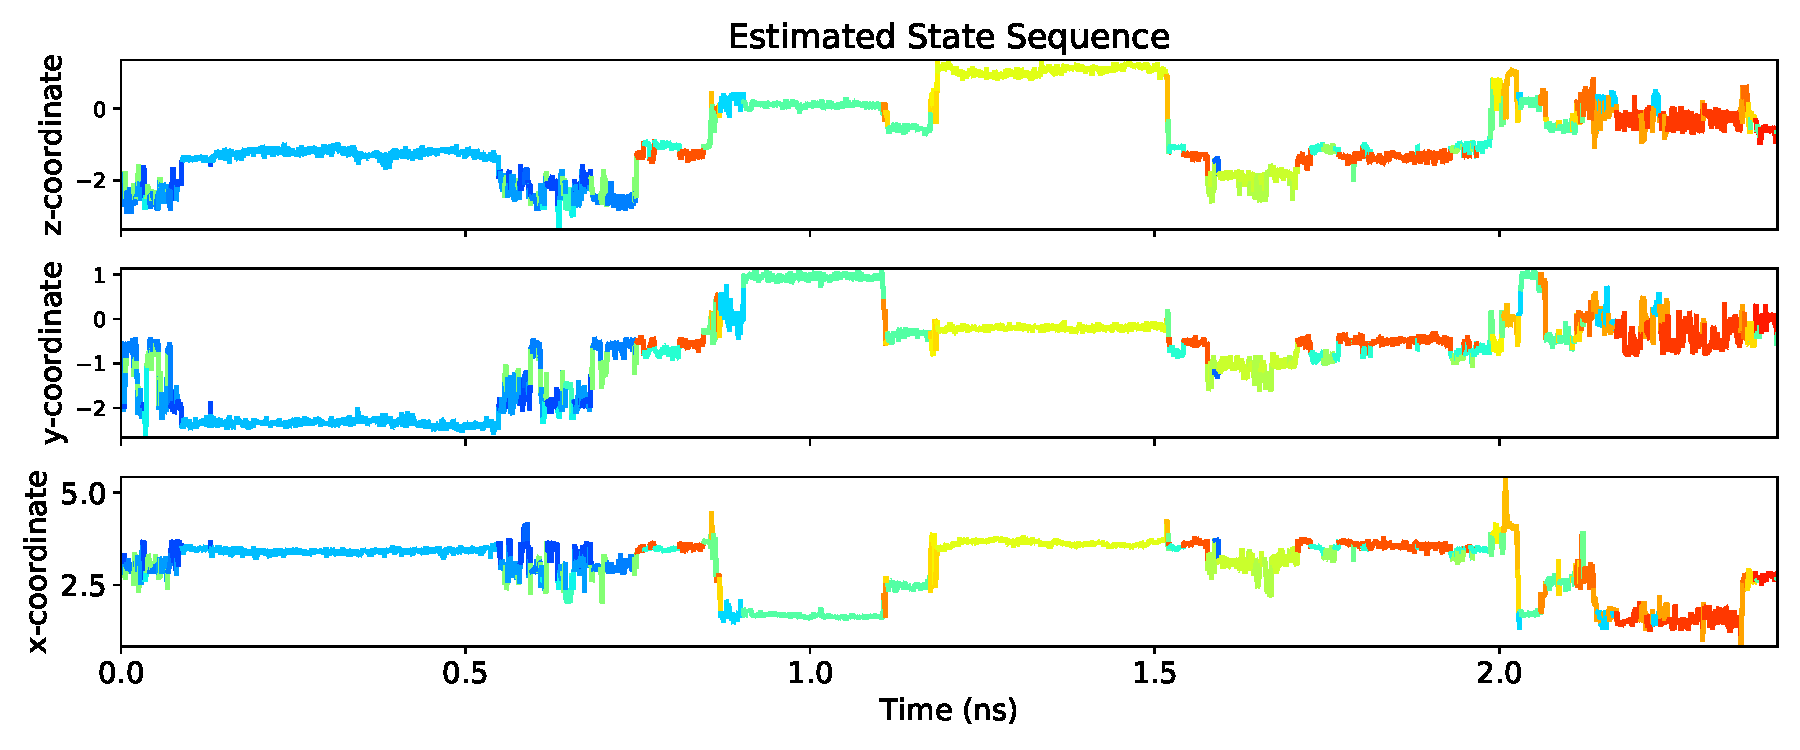
\includegraphics[width=\textwidth]{xyz_hmm.pdf}
		\caption{}\label{fig:xyz_hmm}
	\end{subfigure}  	
	\begin{subfigure}{0.8\textwidth}
		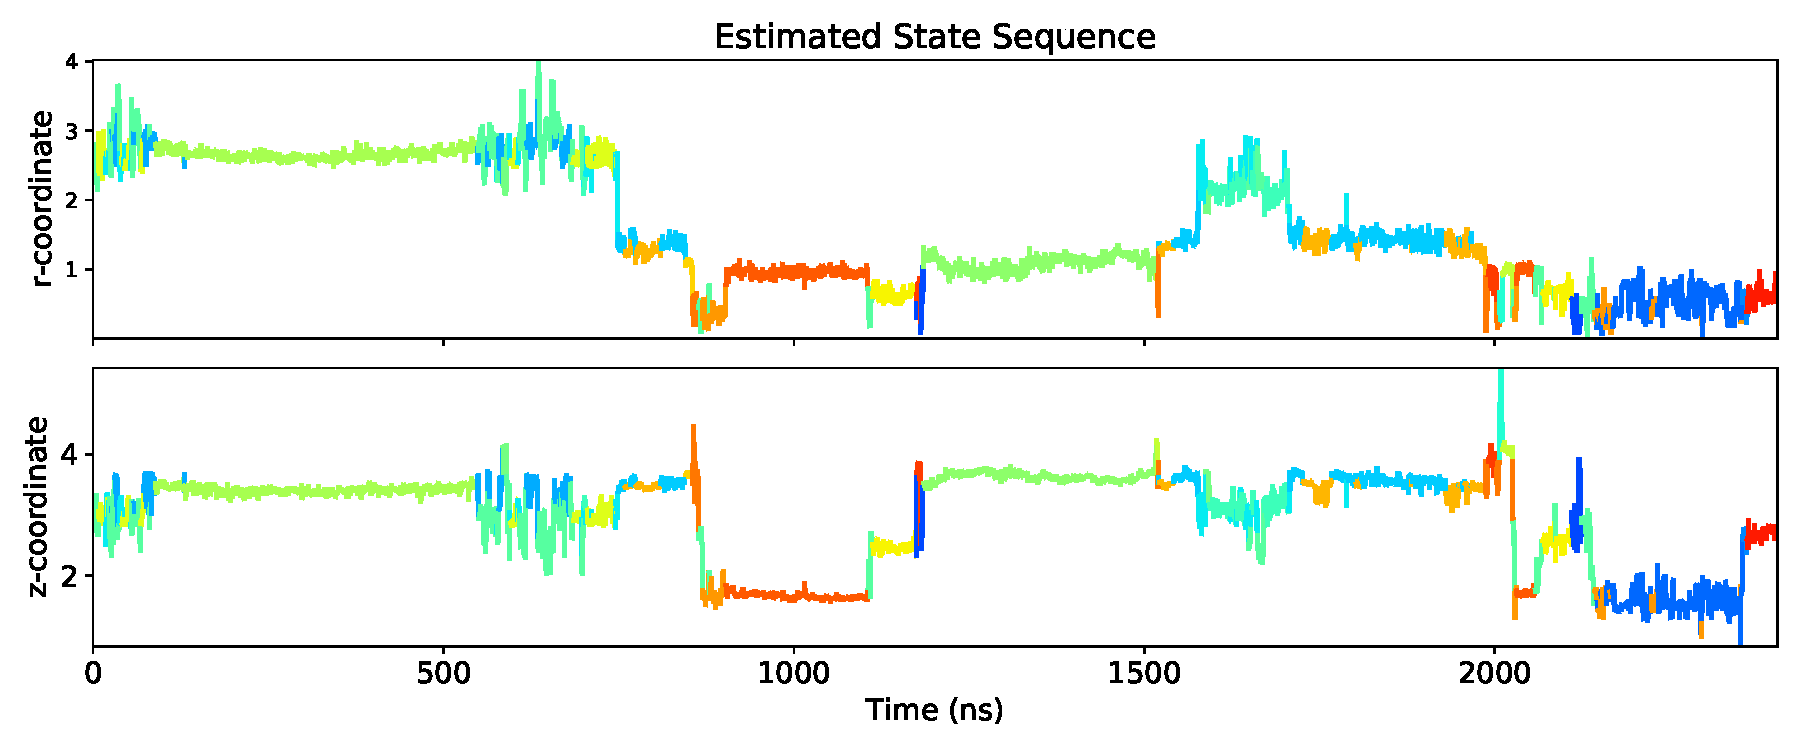
\includegraphics[width=\textwidth]{rz_hmm.pdf}
		\caption{}\label{fig:rz_hmm}
	\end{subfigure}  
	\begin{subfigure}{0.8\textwidth}
		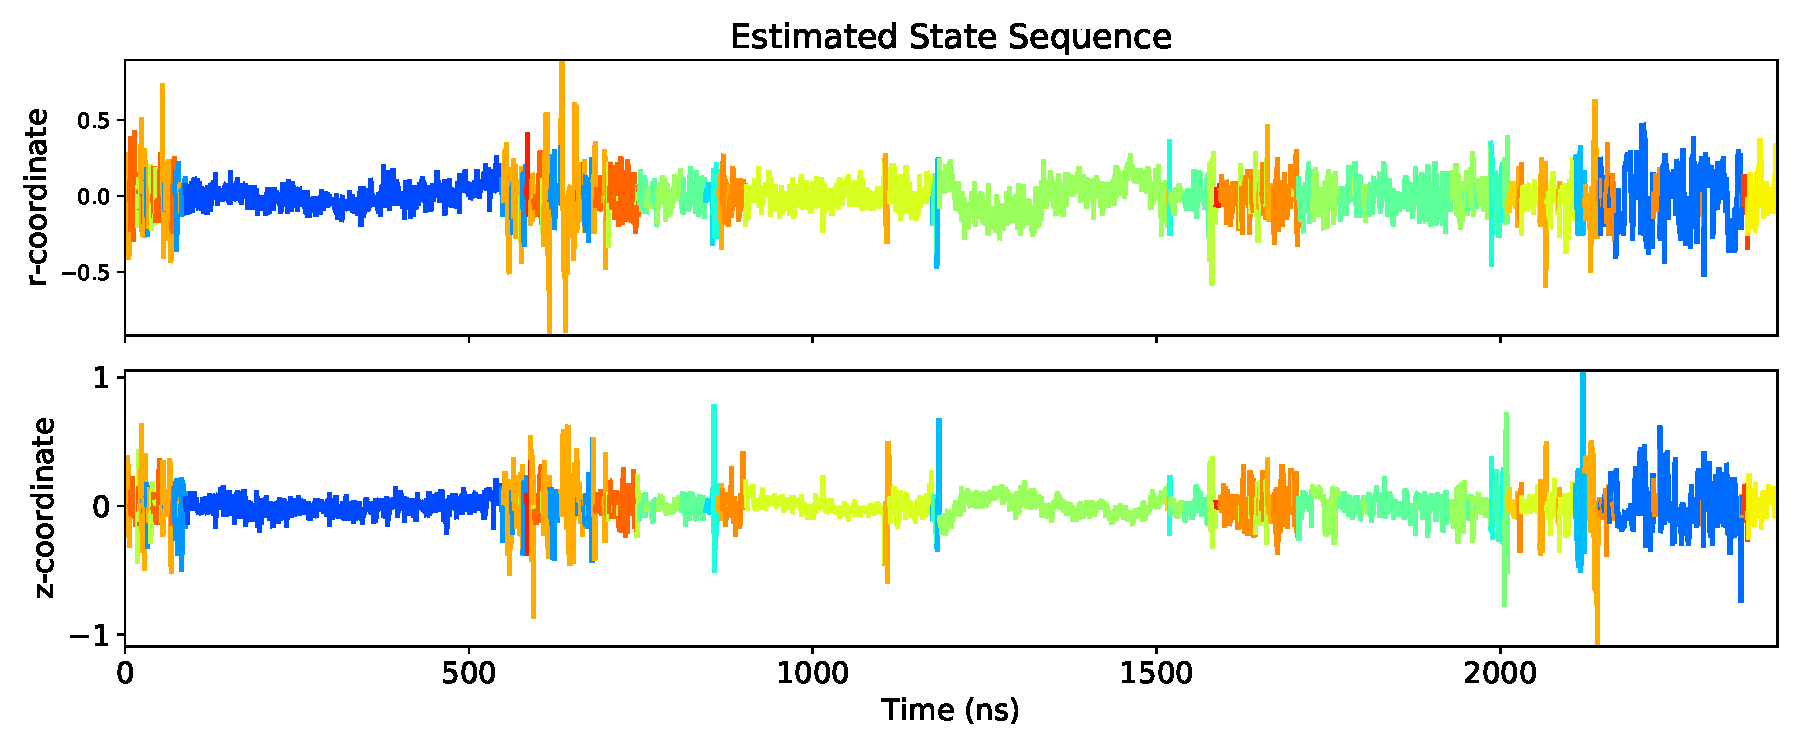
\includegraphics[width=\textwidth]{zeroed_hmm.pdf}
		\caption{}\label{fig:zeroed_hmm}
	\end{subfigure}  
	\caption{IHMM parameterization is a multi-step procedure. In the above plots, distinct colors
	correspond to distinct state behavior. (a) First we parameterize the trajectories in terms of
	the $x$, $y$, $z$ solute center-of-mass coordinates with the $x$ and $y$ coordinates relative
	to the nearest pore center (b) Next, we convert the $x$ and $y$ 	
	coordinates to radial coordinates, $r$, then fix the state sequence and use the inference 
	component of the IHMM in order to estimate the parameters in terms of $r$ and $z$. Note that
	the segment colors in (b) are the same as (a) because we fixed the state sequence.
	(c) After clustering the VAR parameters and reassigning the state sequence so that segments 
	which belong to the same cluster are labeled the same across all solute trajectories, we subtract
	the mean of each segment, obtained before clustering, in order to zero out the
  	trajectory, and then fix the clustered state sequence to infer the parameters of each clustered 
  	state, assuming a mean of zero for all states. Note that the colors are no longer aligned with 
  	figures (a) and (b) because the states are relabeled in terms of their clusters. There are
  	also less states in this single trajectory.
	}\label{fig:hmm_demo}
  \end{figure}
  
  \newpage
  
  \section{Choosing Prior Parameters}\label{section:prior_guesses}  
  
  The states identified by the IHMM are heavily influenced by the Gaussian prior
  placed on $\mathbf{c}$ in Equation~\ref{M-eqn:var} of the main text. The 
  entries of $A$ and $\Sigma$ do not vary over a wide range, so the final
  parameters were relatively insensitive to the priors. In order to 
  maximally automate the IHMM procedure, we attempted to parameterize the
  prior on $\mathbf{c}$ in an intelligent way. The prior parameters should
  be chosen such that the mean level of each state lies within a region of 
  reasonable probability of the prior (see Figure~\ref{fig:prior_guesses}).
  In each dimension, we defined the prior mean to lie halfway between the 
  maximum and minimum of each trajectory dimension. To parameterize the 
  prior's variance in each dimension, we defined the maximum and minimum to 
  be 2 standard deviations from the prior mean. Although this approach has 
  worked quite well for the data in this work, it is important to check the 
  results to determine whether further adjustments to the prior might be needed.
%  In Figure TBD, we show the result of a parameterization where the prior
%  parameters of $c$ were poorly chosen. %TODO
  
  \begin{figure}[h]
  \centering
  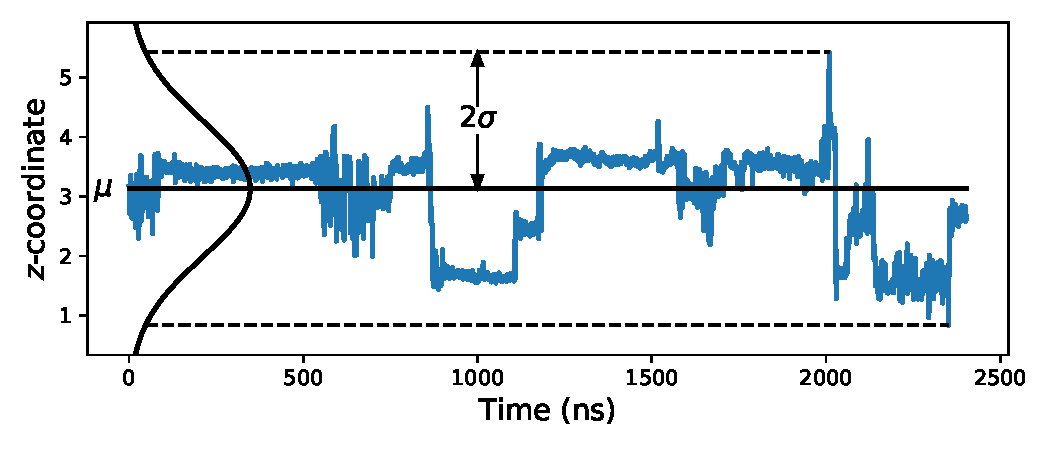
\includegraphics[width=\textwidth]{prior_guesses.pdf}
  \caption{The parameters of the prior on the mean vector, $\mathbf{c}$, (black line), which
  represents the coordinates at which solute are trapped, should be chosen such
  that the mean levels of each state identified in the trajectory (blue line) lie within
  regions of the prior with reasonable probability. We chose the mean of the prior 
  as halfway between the maximum and minimum (shown by the dashed lines) of each trajectory dimension. We chose 
  $\sigma$ of the prior by defining the maximum and minimum to be 2 standard deviations
  from the mean.}\label{fig:prior_guesses}
  \end{figure}
  
  \pagebreak
  
  \section{Parameter Convergence}\label{section:convergence}
  
  The state sequence appears to converge within 500--1000 IHMM iterations. Step 1
  in the procedure from the previous section is the only time the state sequence 
  is determined. We ran 2000 iterations of the IHMM algorithm in order to arrive
  at a finalized state sequence. Stabilization of the VAR parameters indicates 
  that the state sequence has converged. In Figure~\ref{fig:convergence3d}, we plot
  the diagonal entries of 3 different $A$ and $\Sigma$ matrices as well as the 
  entries of the mean vector $\mathbf{c}$, fit to a single 3D methanol trajectory.
  States with a relatively small number of observations are more highly influenced 
  by the boundaries of the state segments and generally lead to much higher 
  variance of the $A$ and $\Sigma$ parameters. In these cases, the mean is
  a more reliable indicator of convergence since stabilized means imply that the
  fluctuations assigned to each state come from motion about a static location.
  
  \begin{figure}[h]
  \centering
  \begin{subfigure}{0.8\textwidth}
  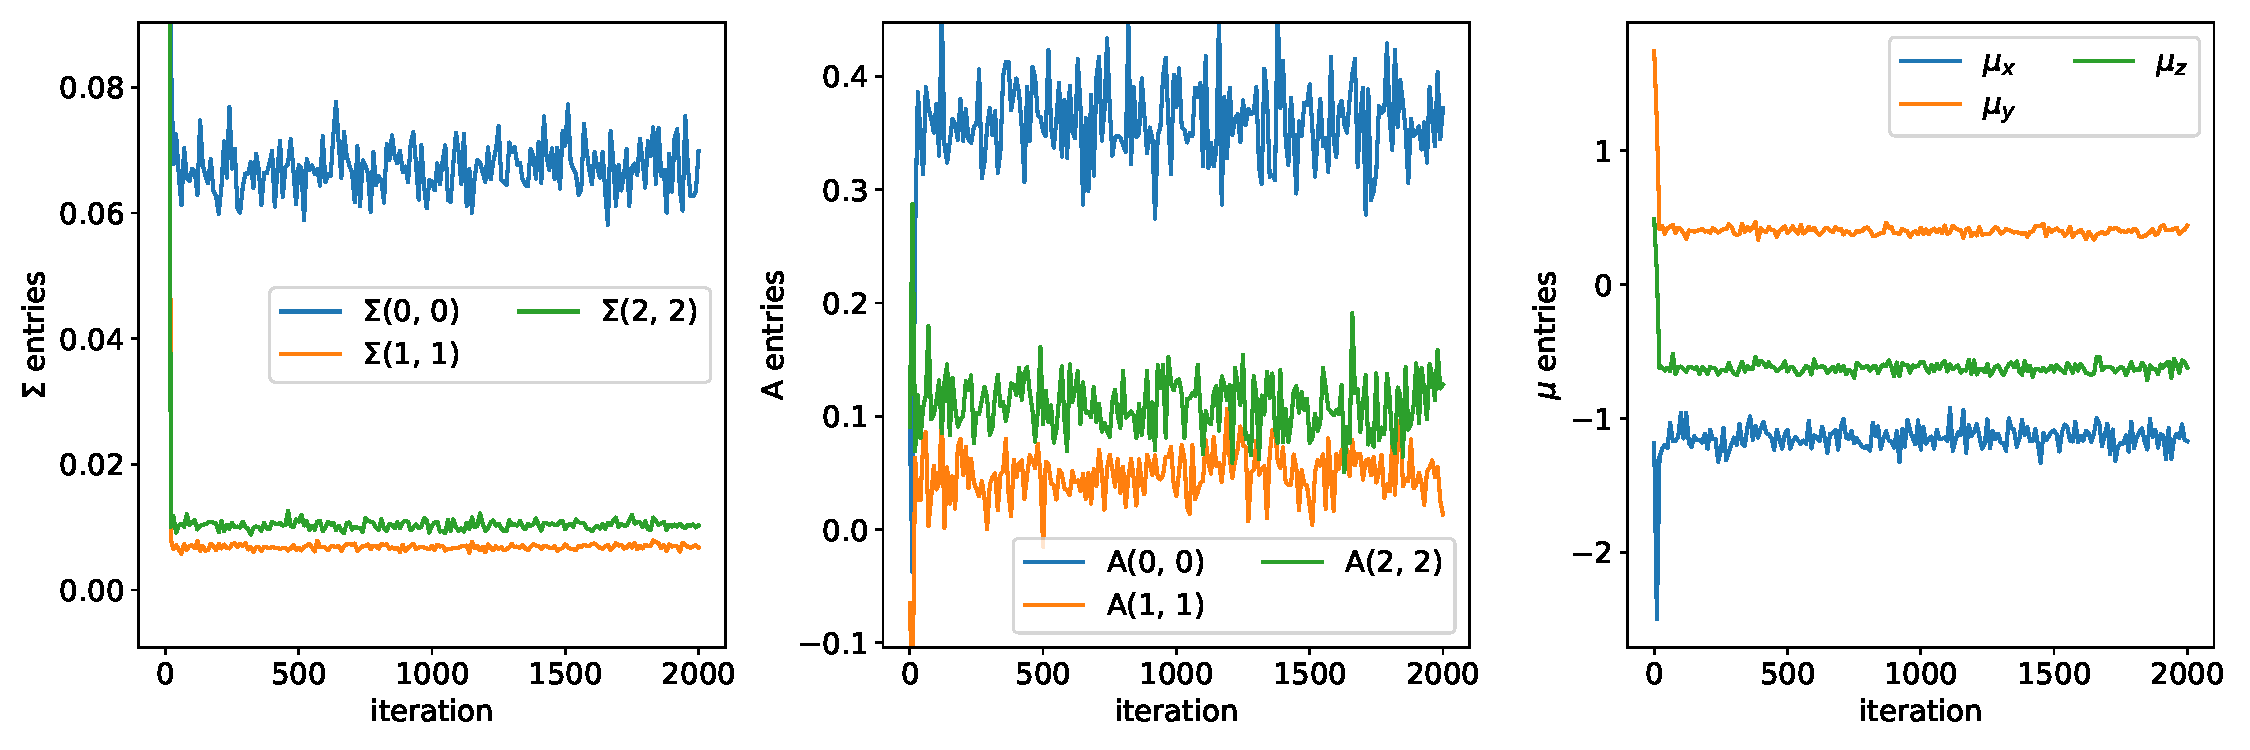
\includegraphics[width=\textwidth]{convergence_MET_47.pdf}
  \caption{706 total emissions}\label{fig:convergence3d_MET_low}
  \end{subfigure}
  \begin{subfigure}{0.8\textwidth}
  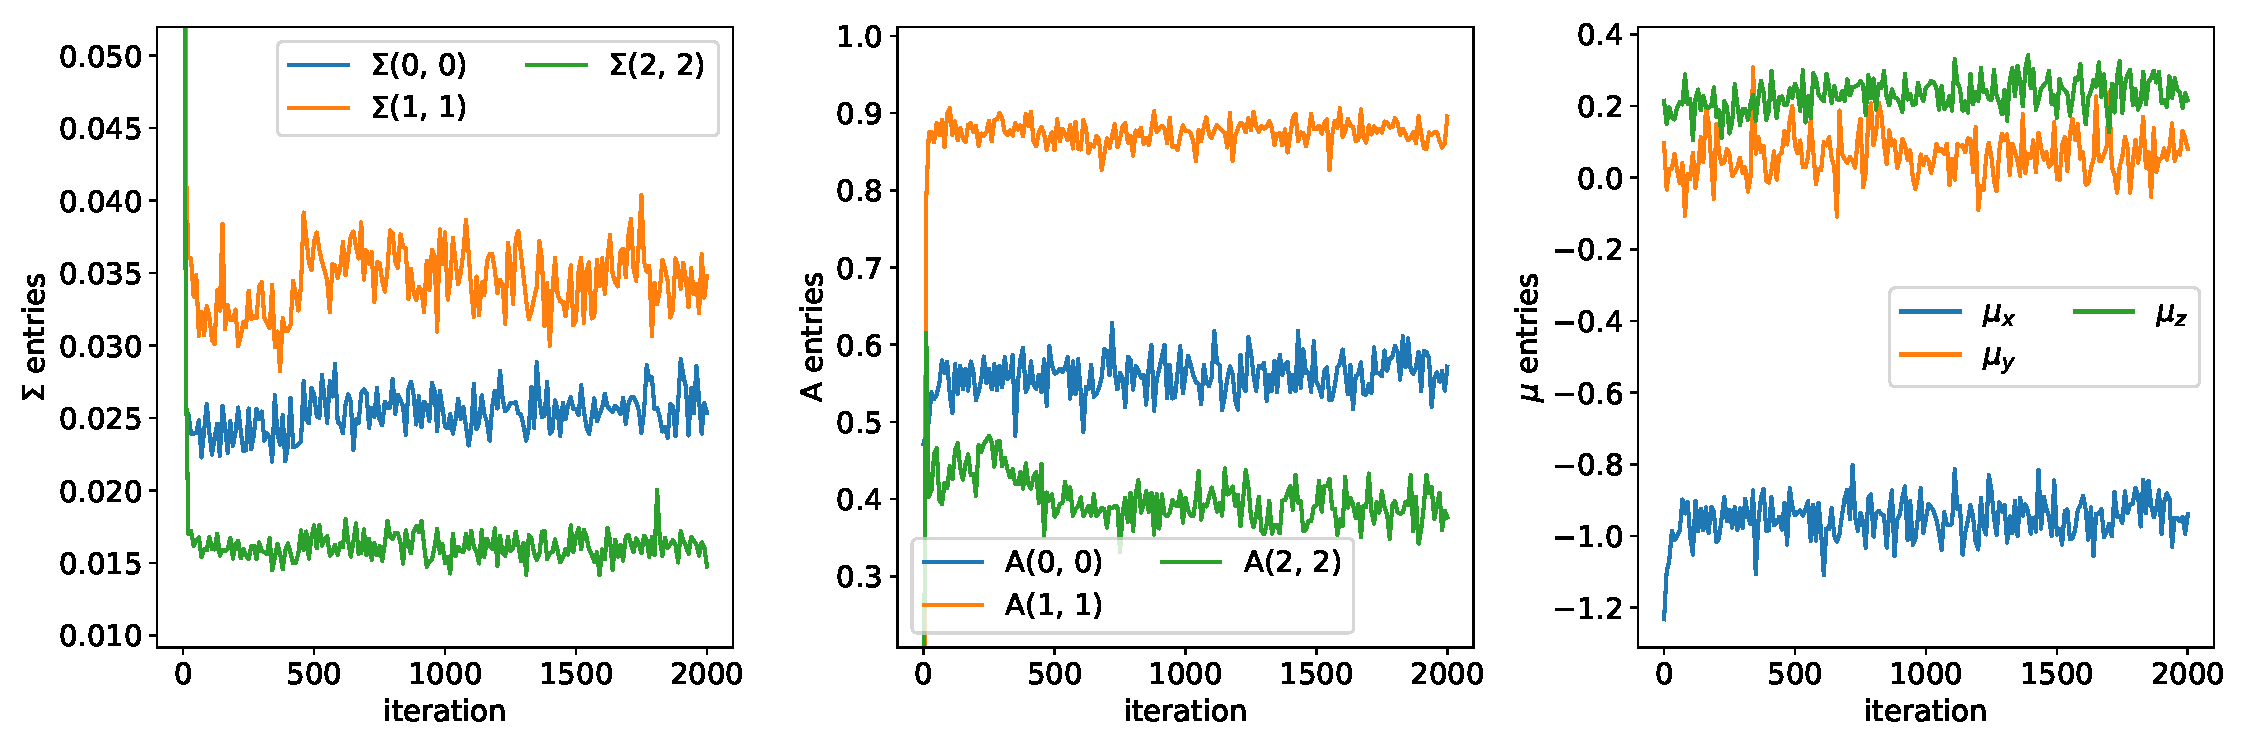
\includegraphics[width=\textwidth]{convergence_MET_36.pdf}
  \caption{1000 total emissions}\label{fig:convergence3d_MET_medium}
  \end{subfigure}
  \begin{subfigure}{0.8\textwidth}
  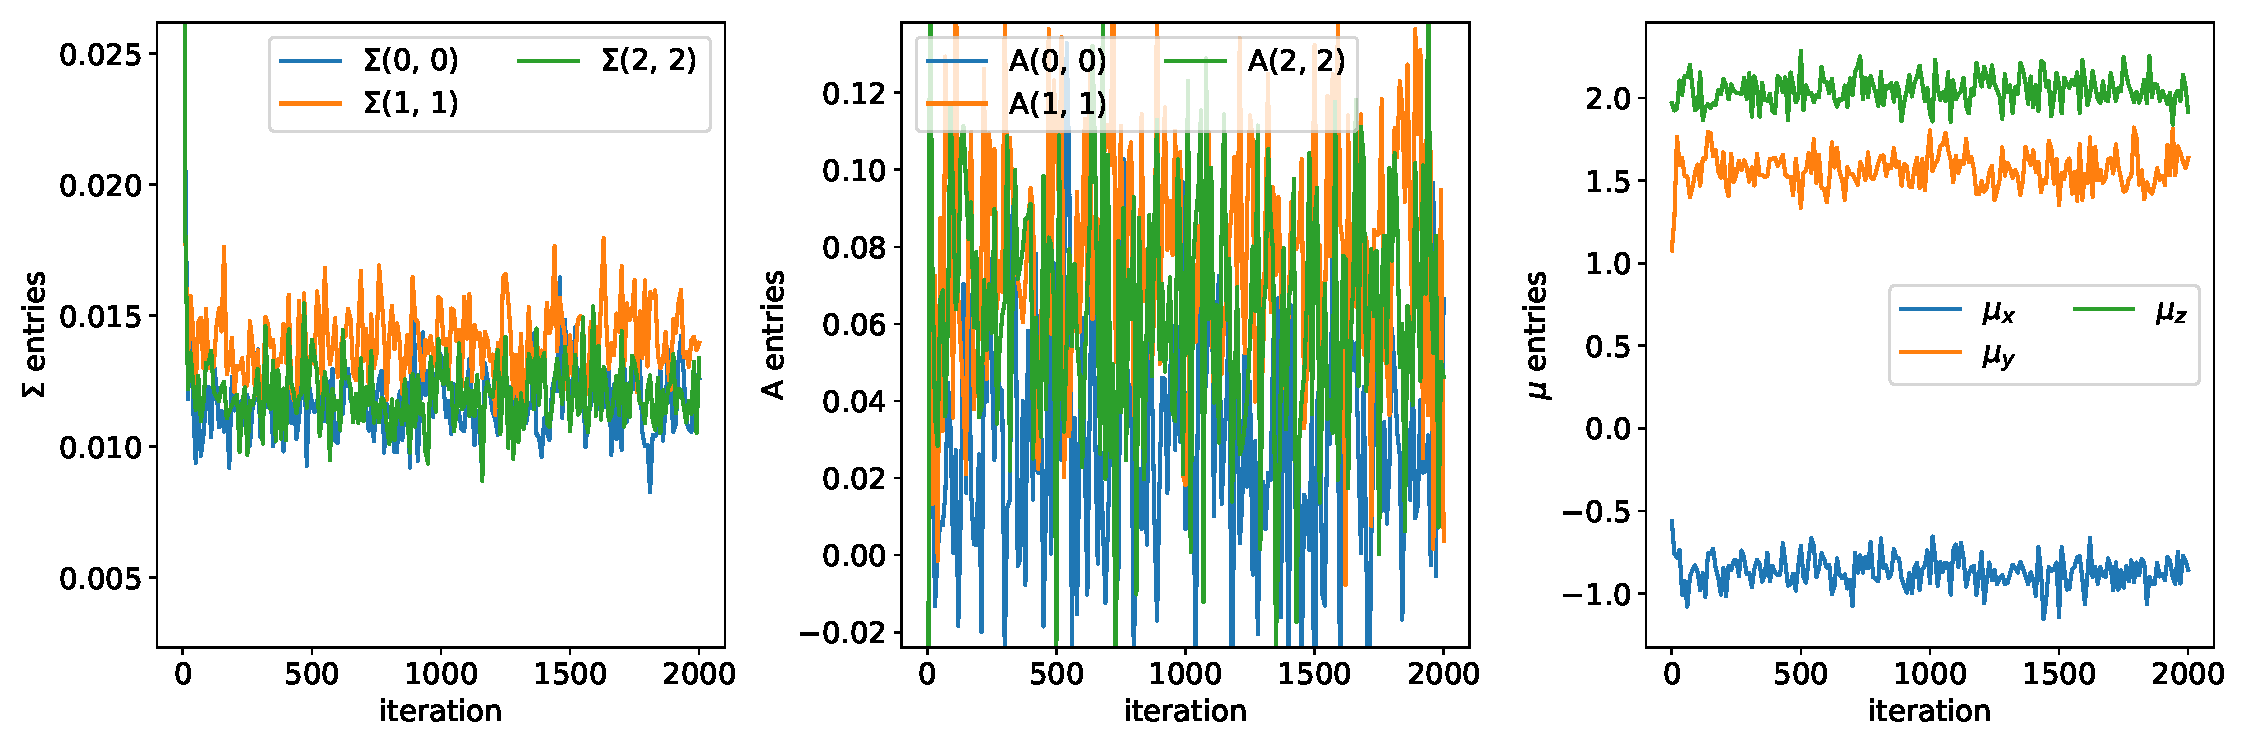
\includegraphics[width=\textwidth]{convergence_MET_59.pdf}
  \caption{201 total emissions}\label{fig:convergence3d_MET_high}
  \end{subfigure}
  \caption{Given a sufficient number of observations for a given mode, the VAR parameters
  appear to converge within 500 -- 1000 iterations. States with too few observations
  are more highly influenced by the boundaries of the state segments and generally
  lead to much higher fluctuations in the VAR parameters.}\label{fig:convergence3d}
  \end{figure}
  
  \clearpage
  
  When we fix the state sequence in subsequent steps of the procedure, parameter 
  estimates converge within only a few steps. In Figure~\ref{fig:fixed_state_convergence}, we 
  plot the entries of $A$ and $\Sigma$ as a function of IHMM iteration. Some states
  are sampled far more frequently than others. High sampling frequently results in
  higher certainty converged parameter estimates. Due to fast convergence, we only
  run 100 iterations of the inference behavior when the state sequence is fixed.
  
  \begin{figure}[h]
  \centering
  \begin{subfigure}{0.6\textwidth}
  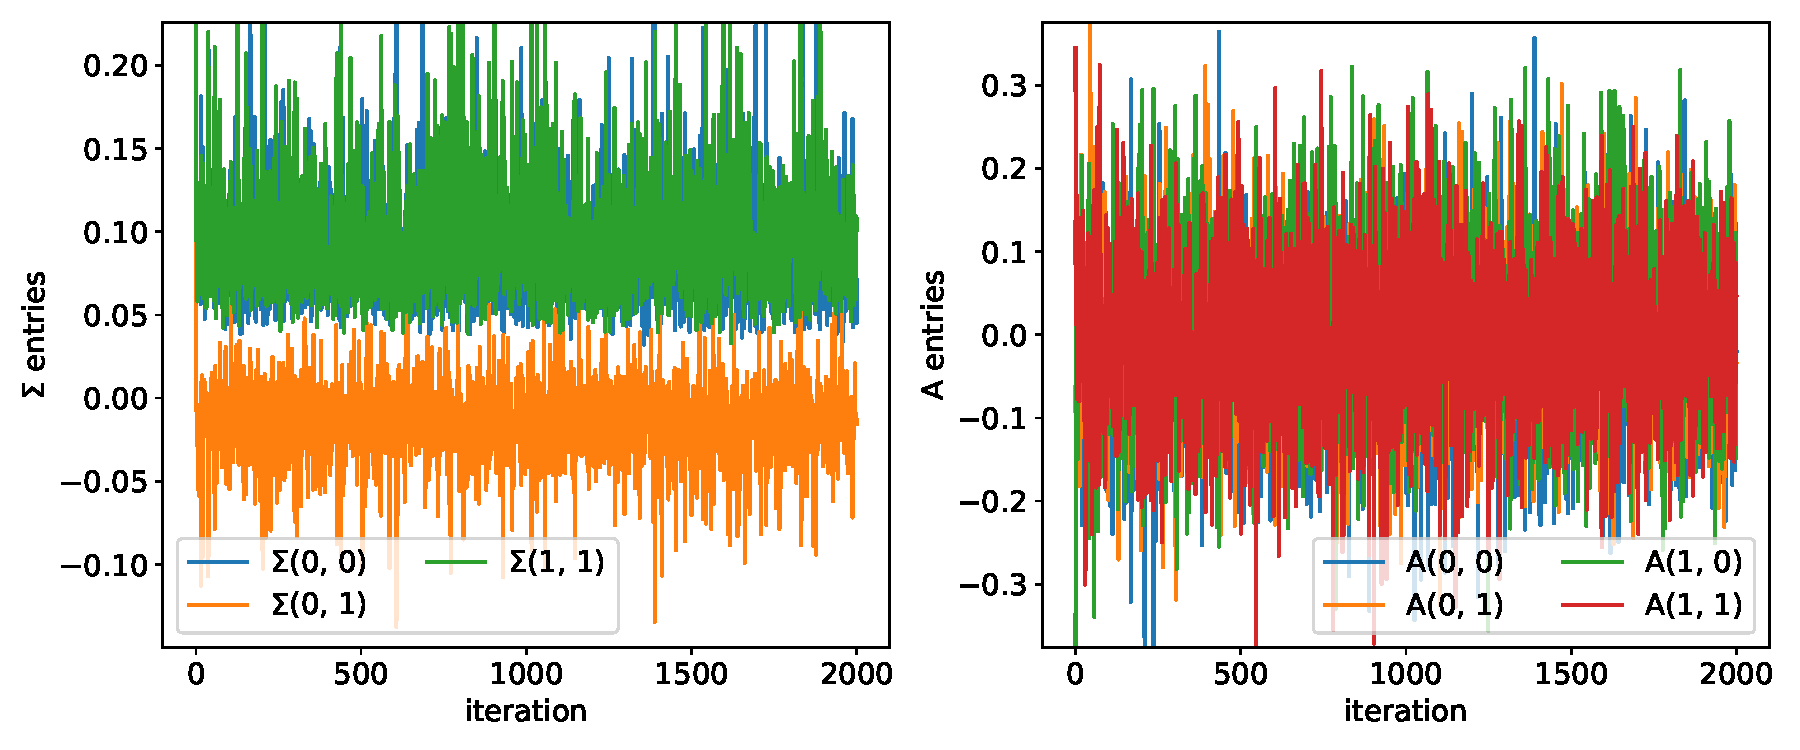
\includegraphics[width=\textwidth]{convergence_MET_4.pdf}
  \caption{15 total emissions}\label{fig:convergence_MET_low}
  \end{subfigure}
  \begin{subfigure}{0.6\textwidth}
  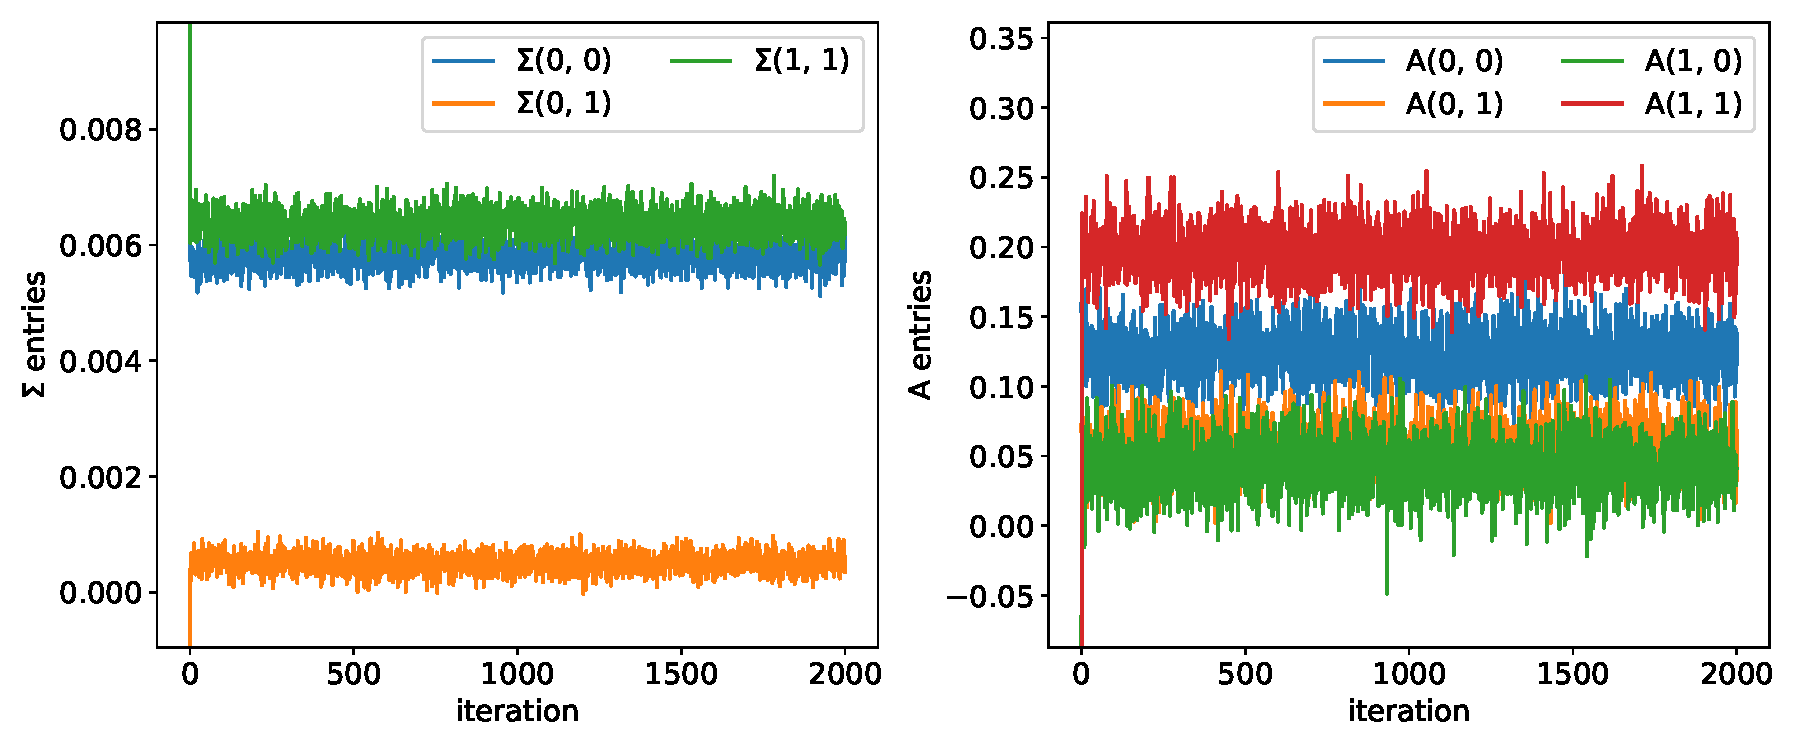
\includegraphics[width=\textwidth]{convergence_MET_21.pdf}
  \caption{1289 total emissions}\label{fig:convergence_MET_medium}
  \end{subfigure}
  \begin{subfigure}{0.6\textwidth}
  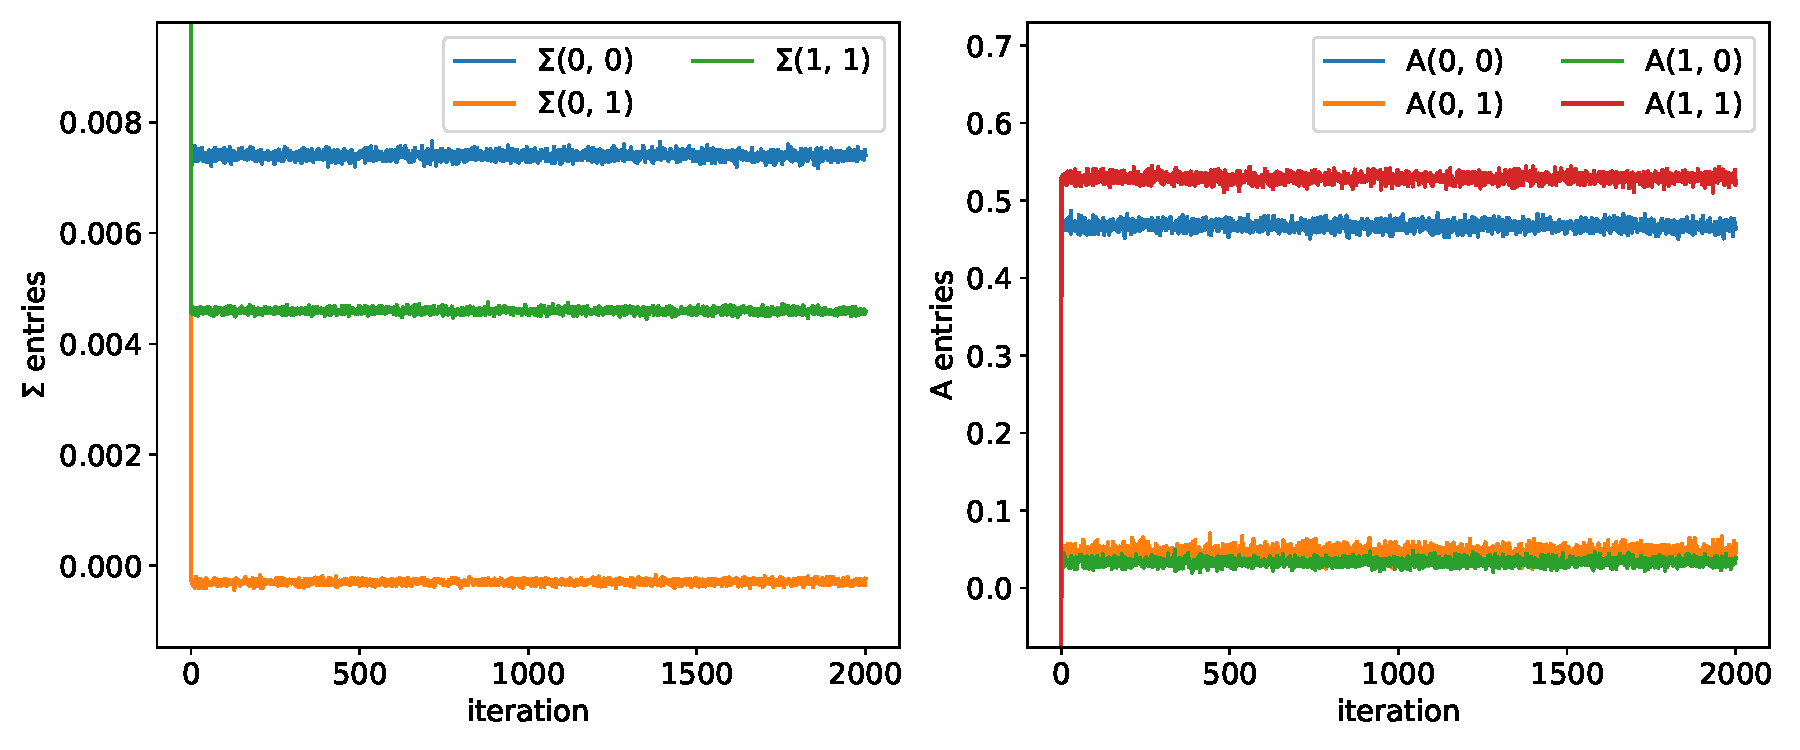
\includegraphics[width=\textwidth]{convergence_MET_15.pdf}
  \caption{24468 total emissions}\label{fig:convergence_MET_high}
  \end{subfigure}
  \caption{The VAR parameters converge quickly when we fix the state
  sequence. As the total number of emissions observed from each state
  increases, the uncertainty in the converged parameters estimates
  decreases.}\label{fig:fixed_state_convergence}
  \end{figure}
  
  \clearpage
  
  \section{Agglomerative Clustering Versus Gaussian Mixture Models}\label{section:agglomerative}
  
  % BJC: will show Gaussian mixture model which has a cluster engulfing another cluster, so
  % it's tails are on both sides of the center cluster.
  
  \begin{figure}[h]
  \centering
  \begin{subfigure}{0.95\textwidth}
  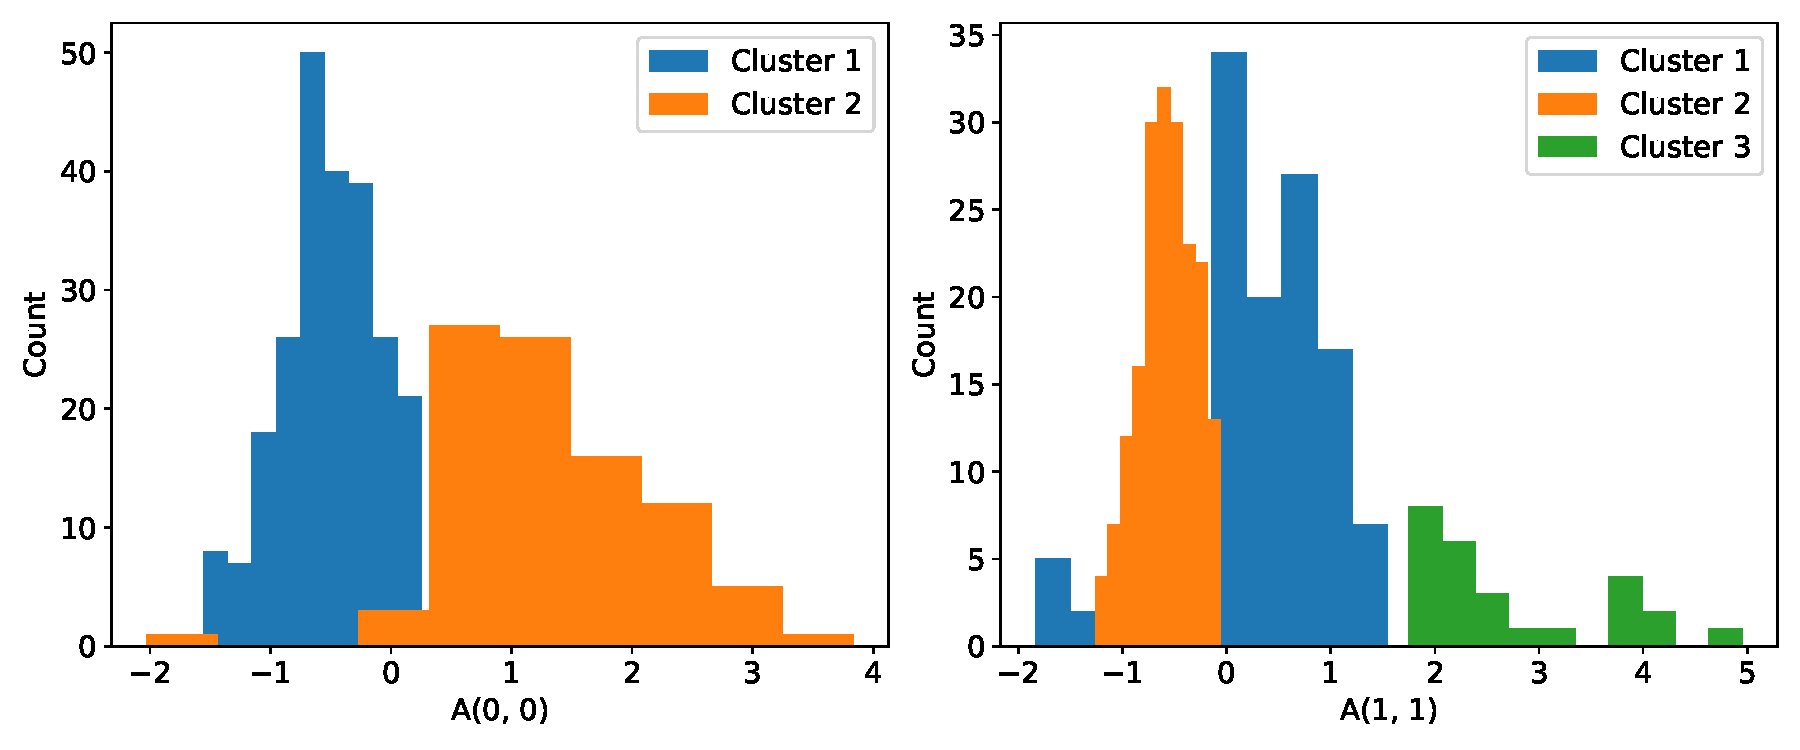
\includegraphics[width=\textwidth]{bayesian_A.pdf}
  \caption{Bayesian Gaussian mixture model}\label{fig:bayesian_A}
  \end{subfigure}
  \begin{subfigure}{0.95\textwidth}
  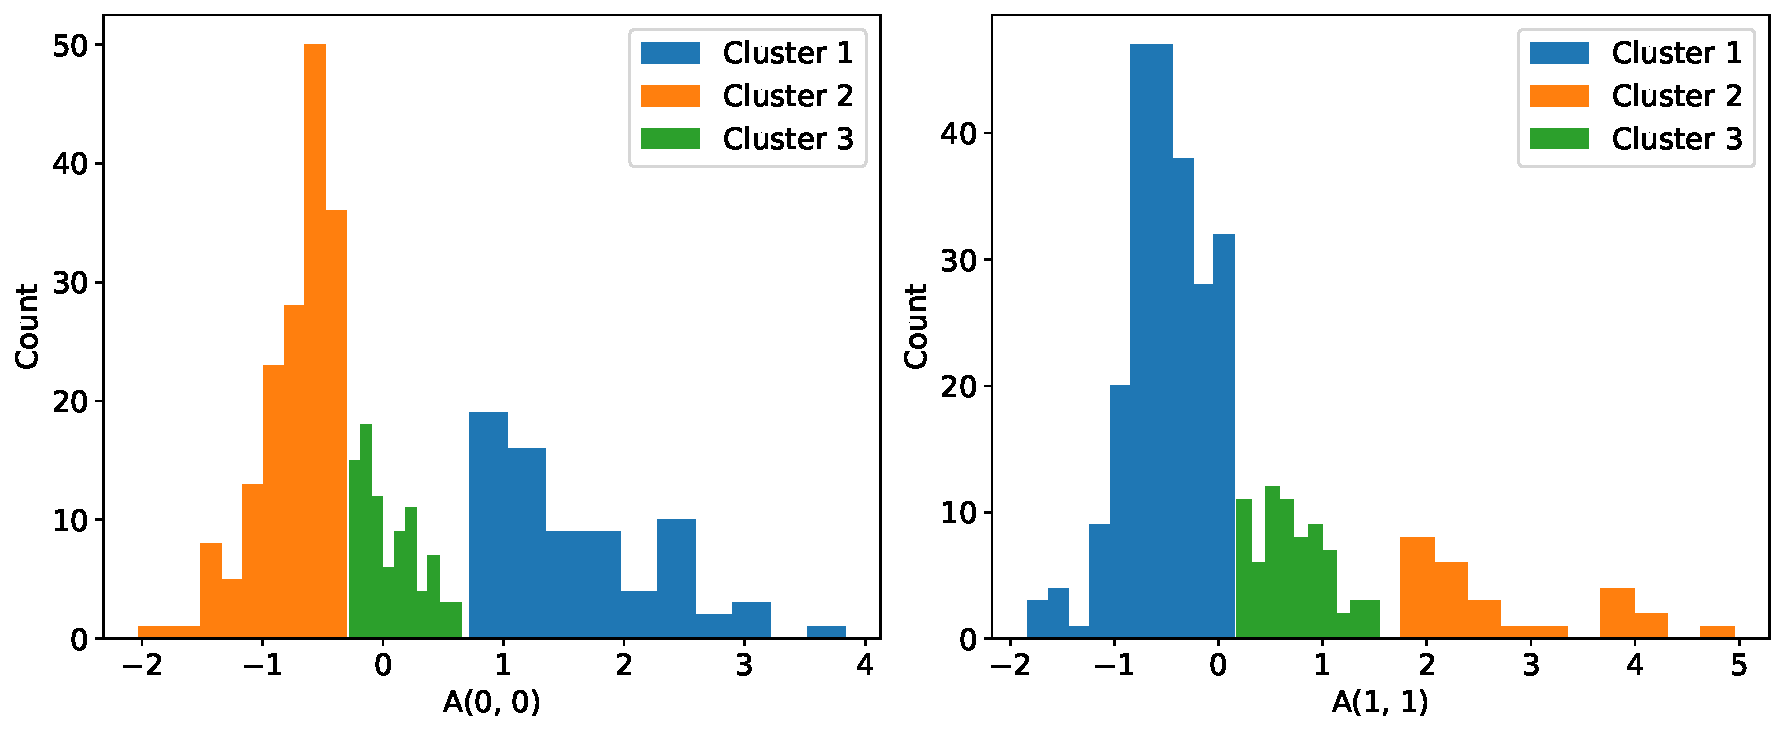
\includegraphics[width=\textwidth]{agglomerative_A.pdf}
  \caption{Agglomerative Clustering}\label{fig:agglomerative_A}
  \end{subfigure}
  \caption{To reduce the state space, we prefer agglomerative clustering over Bayesian
  Gaussian mixture modeling. In the plots above we show the results of clustering the
  diagonal entries of the autoregressive coefficient matrices, $A$, of methanol. (a) 
  Bayesian Gaussian mixture models tend to delocalize the clusters in parameter space
  since the Gaussians can overlap. Agglomerative clustering prevents overlap of 
  clusters and ensures that all states within each cluster have similar parameters.
  }\label{fig:clustering_choice}
  \end{figure}
  
  \newpage
  
  \section{Choosing the Number of Clusters}\label{section:nclusters}
  
  \begin{figure}[h]
  \centering
  \begin{subfigure}{0.45\textwidth}
  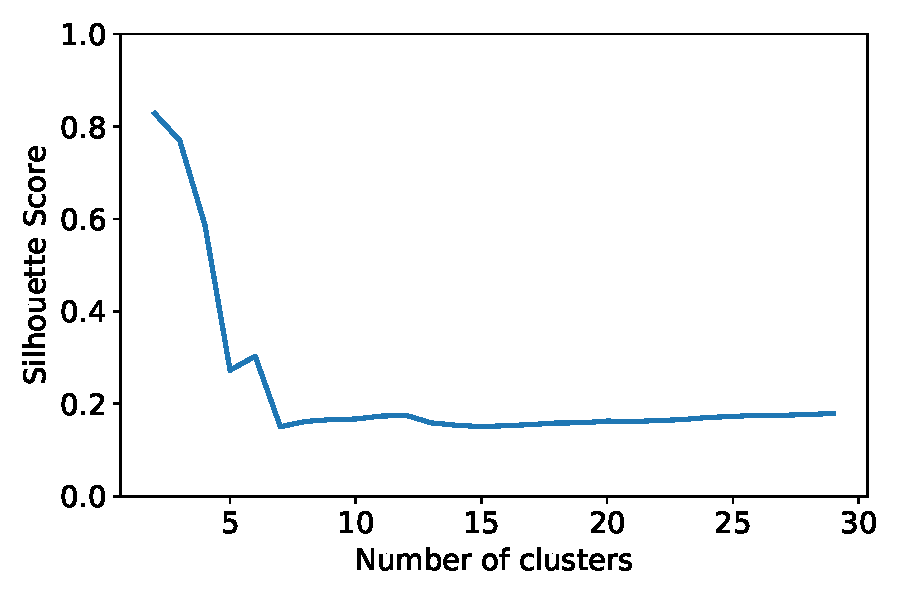
\includegraphics[width=\textwidth]{silhouette_MET.pdf}
  \caption{methanol}\label{fig:silhouette_MET}
  \end{subfigure}
  \begin{subfigure}{0.45\textwidth}
  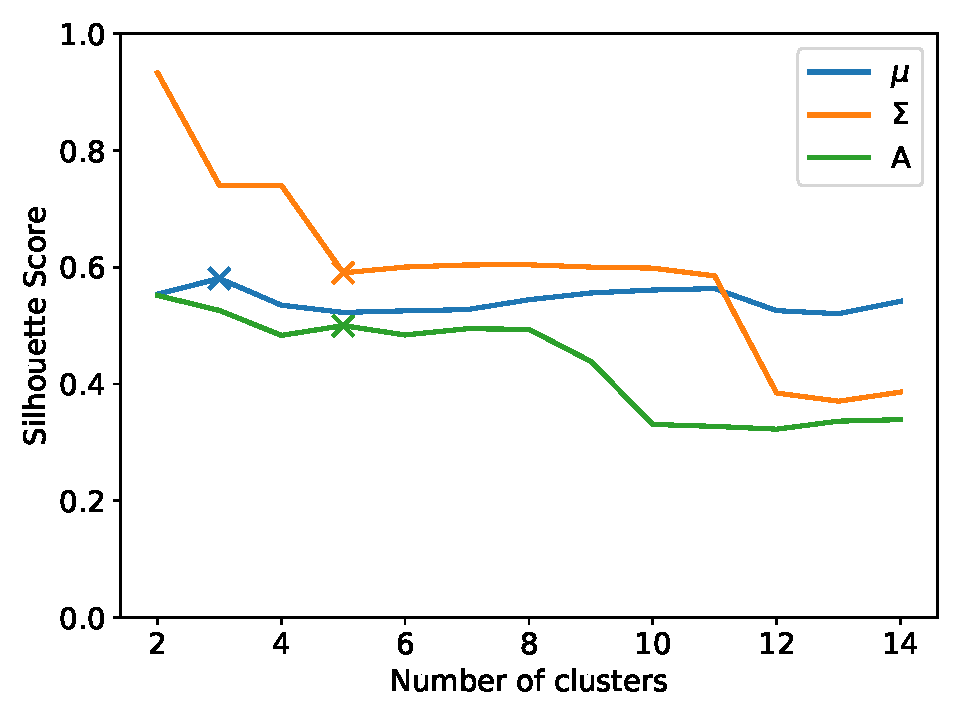
\includegraphics[width=\textwidth]{silhouette_URE.pdf}
  \caption{urea}\label{fig:silhouette_URE}
  \end{subfigure}
  \begin{subfigure}{0.45\textwidth}
  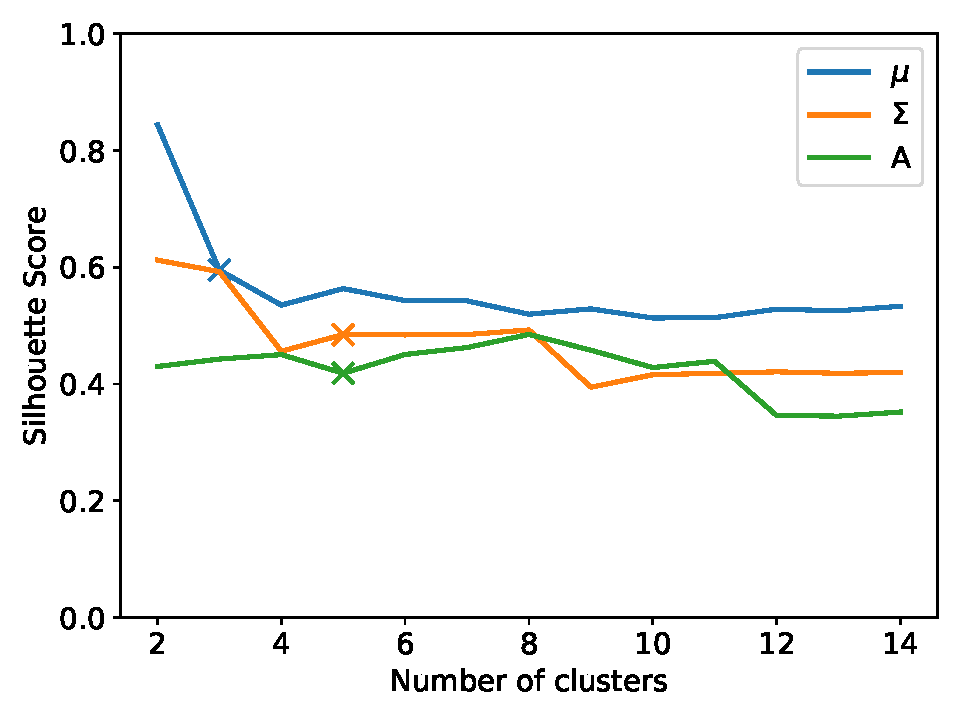
\includegraphics[width=\textwidth]{silhouette_GCL.pdf}
  \caption{ethylene glycol}\label{fig:silhouette_GCL}
  \end{subfigure}
  \begin{subfigure}{0.45\textwidth}
  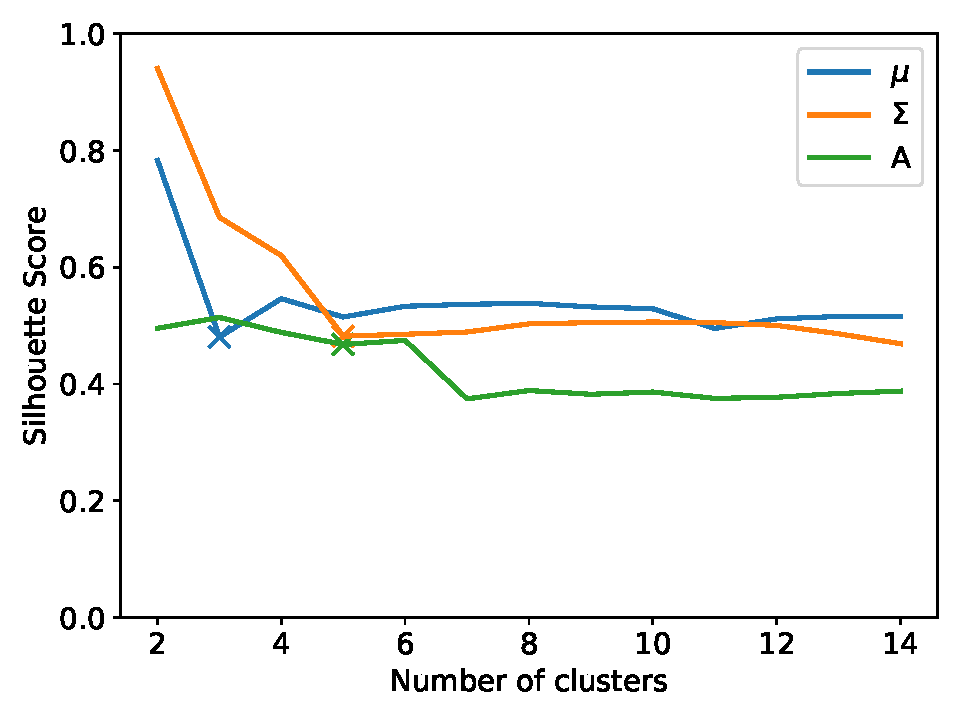
\includegraphics[width=\textwidth]{silhouette_ACH.pdf}
  \caption{acetic acid}\label{fig:silhouette_ACH}
  \end{subfigure}
  \caption{We used the silhouette score test in order to quantitatively
  inform our decision on the numbrer of clusters. Silhouette scores 
  closer to one indicate good clustering. The crosses on the plot indicate
  our choice in number of clusters after careful consideration of the
  silhouette scores in conjunction with qualitative examination of the clusters
  formed by the choice. Although the test often
  favors fewer states, we elected to use an intermediate number of states in 
  the cases of $A$ and $\Sigma$ because choosing 2--3 clusters 
  insufficiently separates the dynamical modes. }\label{fig:silhouette}
  \end{figure}
  
\end{document}